\chapter{Requirements}
\label{chap:requirements}

% Beginning of the document
\section{Introduction}

This document aims to define the specifications of the \emph{Cracked records with 3D/IRENE} Master Thesis. It describes the main project objectives and specifies the needed tasks.

The important milestones during the semester are also defined.

\section{Context}

IRENE and 3D Probe are solutions maintained by Carl Haber and his team at the Lawrence Berkeley National Laboratory (LBNL). They consist of hardware and software which are able to recover the sound information from different types of old records without physical contact. The first system uses a common camera to scan the records while the second one uses a special 3D probe.

To get the sound information from the acquisition, the two programs called RENE and PRISM read the raw data and output the final processed sound by applying image and signal processing algorithms.

However, with some old material, several problems can happen. One of the most common one is cracked discs, that is, discs that are deteriorated because of the shrinkage of the lacquer layer. The signal is then cut by the cracks, which makes difficult to track the grooves. RENE and PRISM implement already a feature enabling to manually add some points to track the groove, but the solution is still not entirely satisfying because it is slow. It may also be difficult to find manually the correct match when shifts occur.

In a first step, the goal will be to improve the user interface to enhance the manual tracking feature. Then, the final goal will be, in some situations, to be able to automatically track cracked discs or other damaged records by implementing new algorithms in the application.

\section{Objectives}

This section details the main objectives to achieve during the thesis. The secondary objectives are indicative and may be modified over time.

\subsection{Main objectives}
\label{sec:mainobjectives}

\begin{itemize}
    \item Analyze the RENE and PRISM programs to be able to use them in common situation and program new features in the code base.
    \item Analyze the cracked records algorithm in VisualAudio to be able to extend it for the IRENE program. Find out the main differences in VisualAudio compared to the 3D/IRENE systems.
    \item Improve the current manual tracking feature to be more efficient and user-friendly.
    \item Add a new feature able to process some cracked records automatically or helping the user finding the best match by analyzing the signal.
    \item Be able to restore the sample recordings with the tools developed in this project.
    \item Be careful to maintain the application in stable condition and to avoid introducing regression.
\end{itemize}

\subsection{Secondary objectives}

\begin{itemize}
    \item Improve the application code architecture for a good maintainability.
    \item Maintain/improve the code documentation.
\end{itemize}

\section{Tasks}

This section presents the tasks (from the objectives and the initial plan included in \autoref{sec:initstatement}) that have to be planned.

\subsection{Analysis}

\begin{itemize}
    \item RENE and PRISM familiarization and analysis.
    \item Learn the cracked records implementation in VisualAudio and make a presentation of it to the weekly student seminar at LBNL.
    \item Consideration about a more interactive user interface for the manual tracking.
    \item Consideration about the integration/adaptation of the solution implemented in VisualAudio.
    \item Consideration about the possible scaling corrections needed and the gaps caused by the cracks.
\end{itemize}

\subsection{Design/Implementation}

\begin{itemize}
    \item Design and implementation of new GUI features improving the manual tracking.
    \item Design and implementation of an automatic reassembly system for cracked records (correct matching of the shifts).
\end{itemize}

\subsection{Tests}

\begin{itemize}
    \item Functional tests over the test set.
    \item GUI tests.
\end{itemize}

\subsection{Documentation}

\begin{itemize}
    \item Report writing
    \item User documentation
    \item Thesis defense preparation
\end{itemize}

\section{Planning}

\subsection{Important dates}

\begin{description}
\item[2012-09-17] Project start
\item[2012-10-01] Weekly student seminar presentation
\item[2013-02-08] Project end (report restitution)
\item[2013-03-04 to 2013-03-15] Oral defense (in Switzerland, exact date not defined)
\end{description}

\subsection{Gantt Chart}
The tasks appear in the Gantt Chart in \autoref{fig:planning}. The project main milestones are also specified. Nevertheless, this planning is more a general overview than a detailed schedule. Some objectives may be modified in the future regarding the future progress of the project.

\begin{landscape}
%\vspace*{\fill}
\begin{figure}[!h]
\centering
%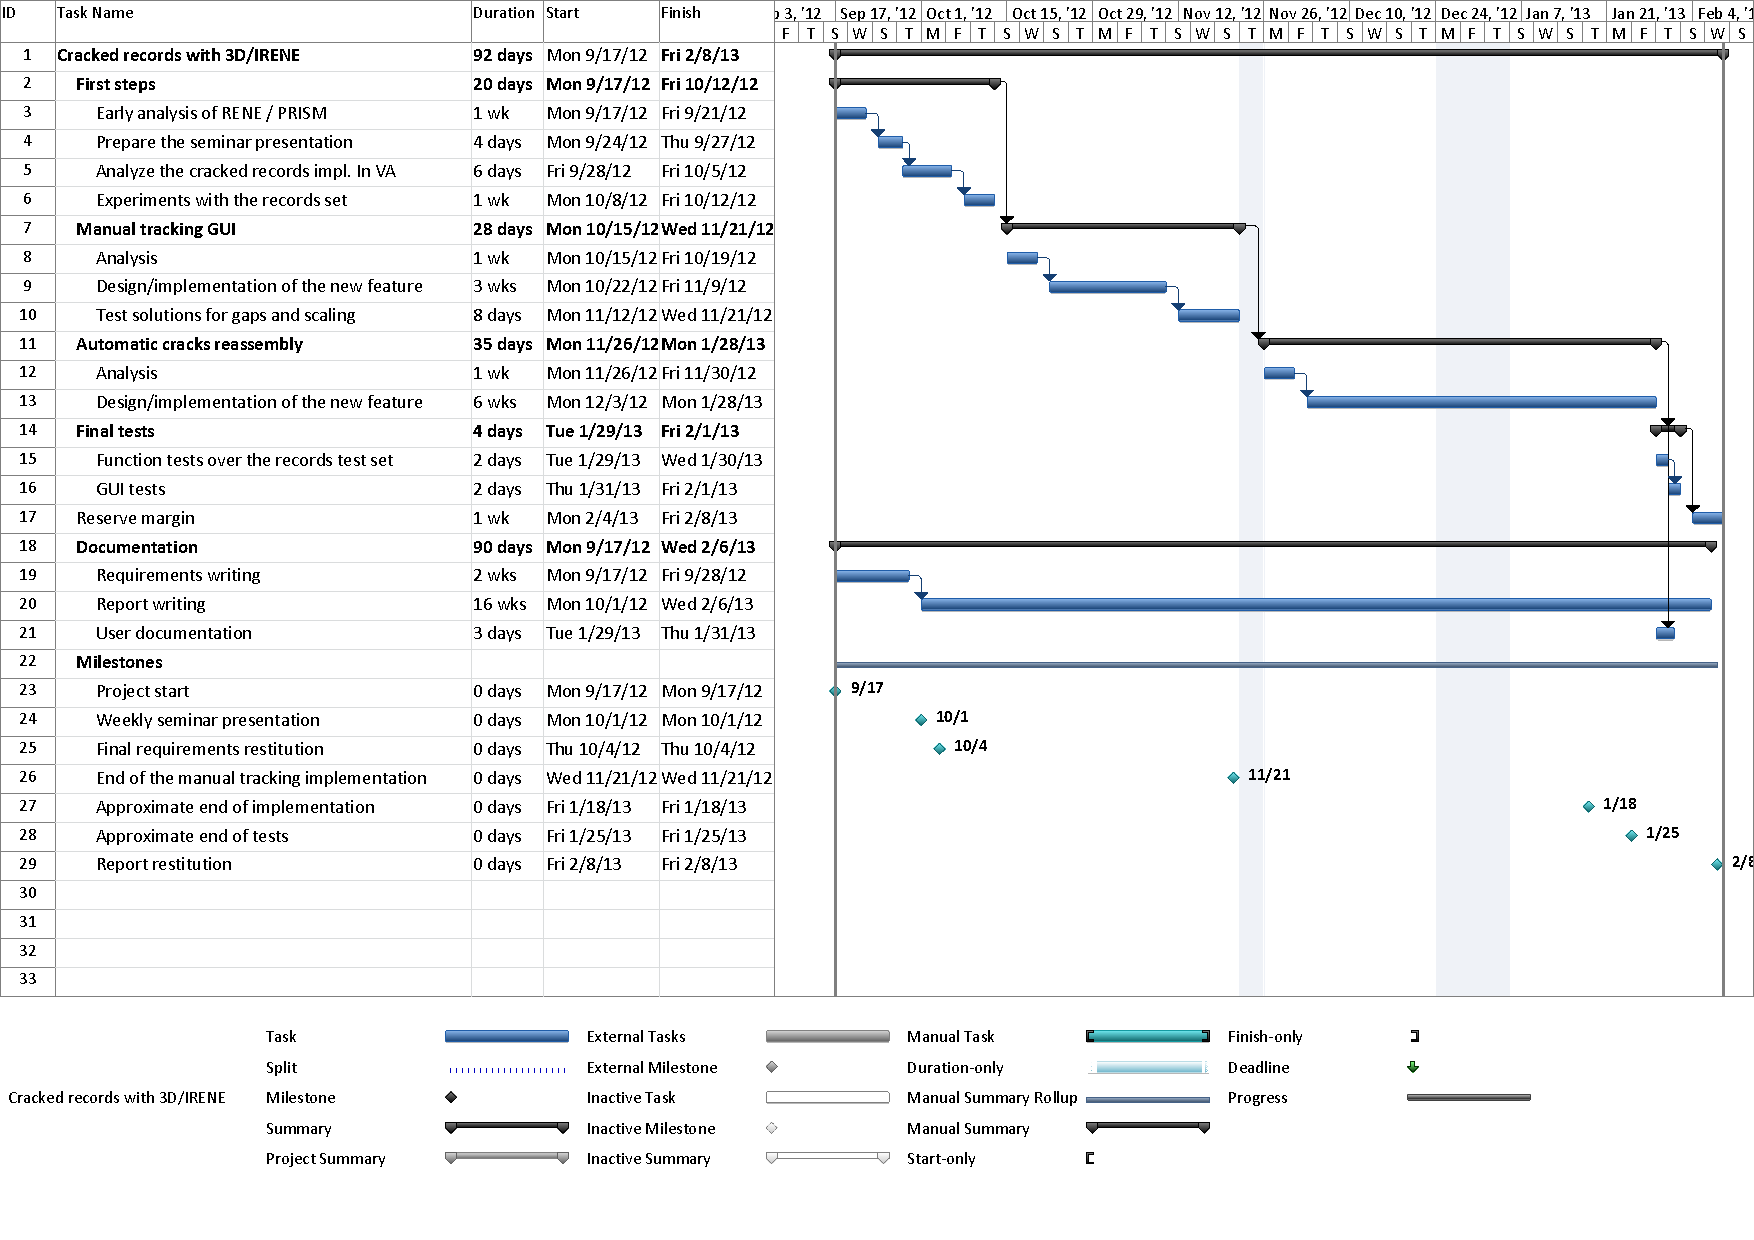
\includegraphics[angle=90,height=18.5cm]{images/planning} 
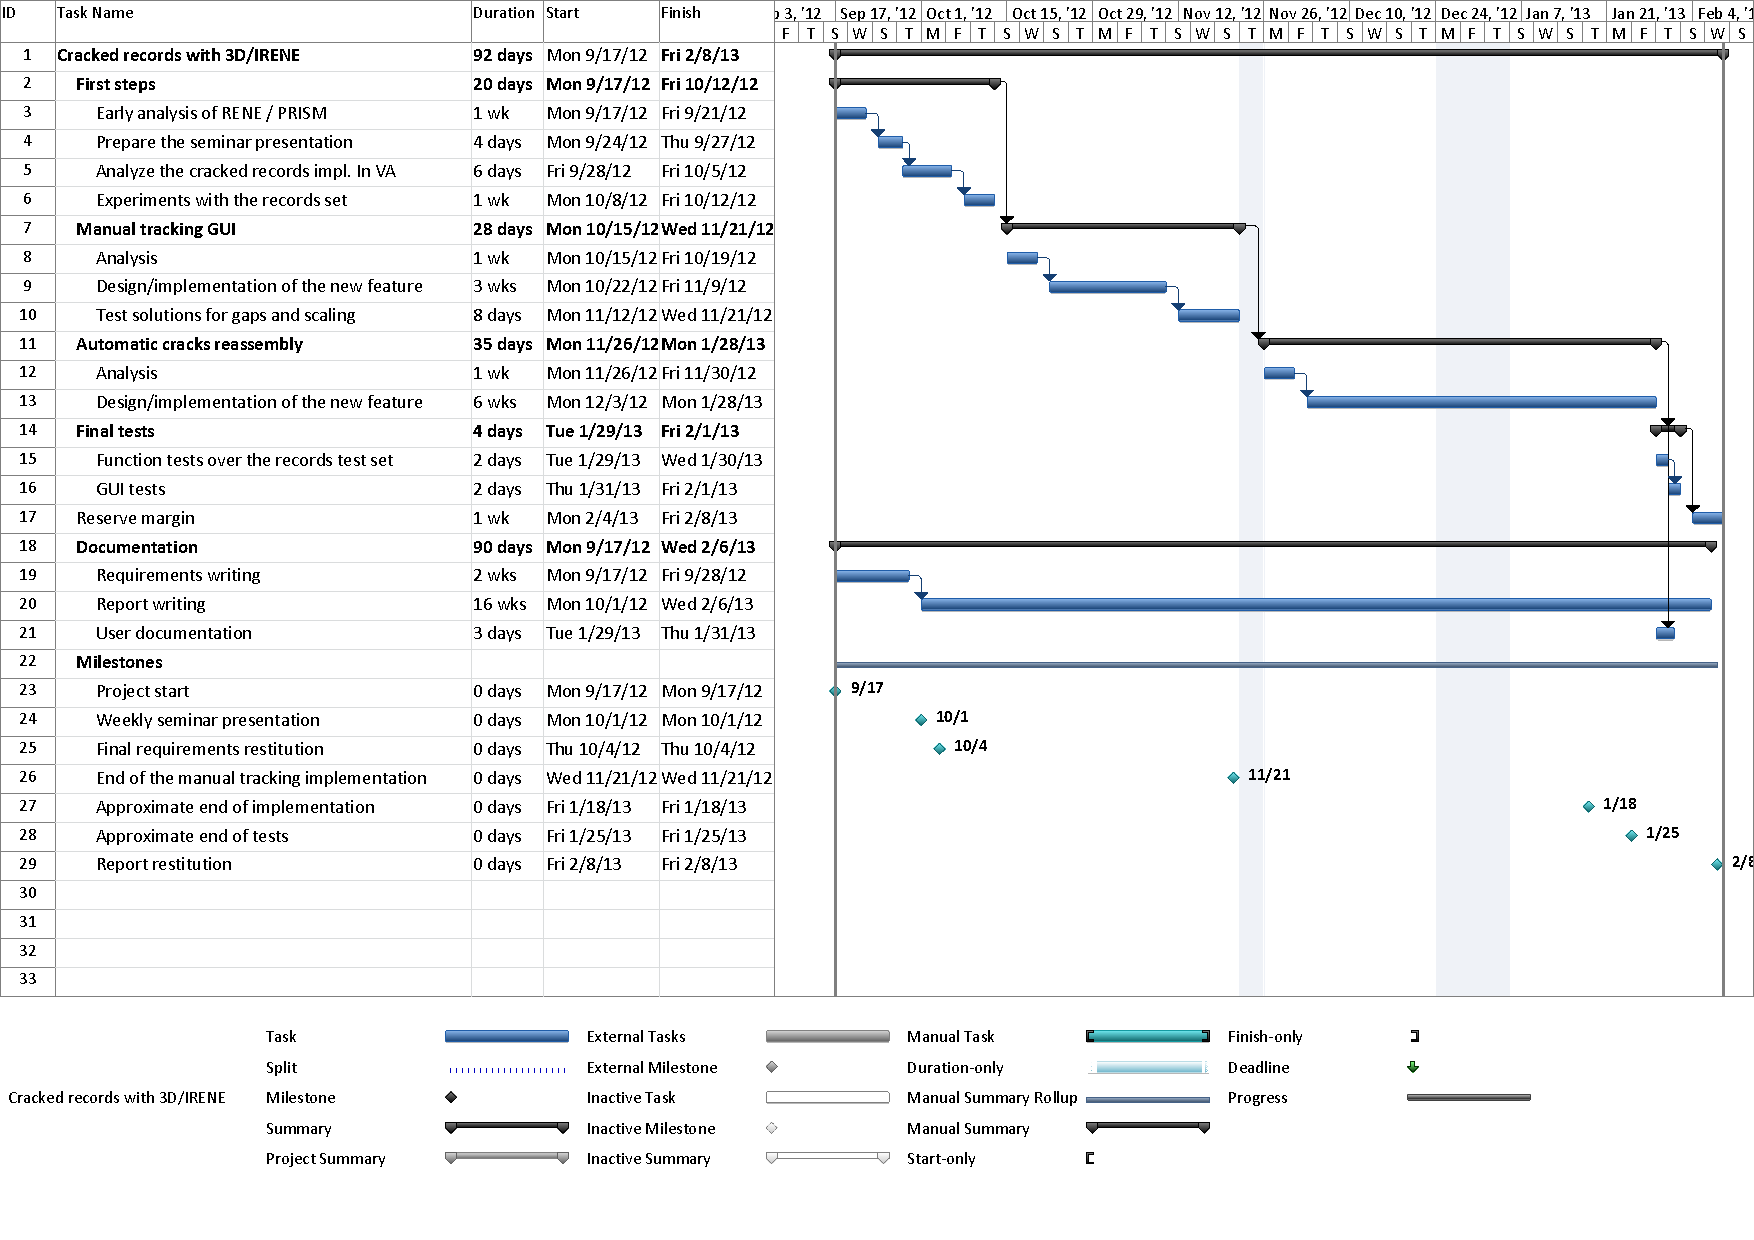
\includegraphics[width=0.95\linewidth]{images/planning} 
\caption{Gantt Chart for the entire schedule of the thesis.}
\label{fig:planning}
\end{figure}
%\vspace*{\fill}
\end{landscape}

\newpage

\section{Initial specifications}
\label{sec:initstatement}

At Lawrence Berkeley National Laboratory, Carl Haber, Earl Cornell, and collaborators have been working on the extraction of sound from phonographic records. They have developed both a 2D (image, referred to as IRENE) and a 3D (depth) system. The proposed project is part of a collaboration between this research team and EIA-FR, who have developed their own solution VisualAudio.

Old disc and cylinder records and other early experimental recordings can suffer from different kinds of degradations. Cracked transcription discs represent a frequent defect: the lacquer coating shrinks, which causes cracks where the plate support (metal or glass) is visible. Wax cylinders are brittle and on occasion break into two or more separate pieces. Early experimental recordings come in a variety of obsolete formats. These include foil sheets, wax discs on a number of different backing materials, metal plated depositions derived from wax masters, and glass discs with photosensitive coatings. Among this variety are many examples of breakage and deformation.

For the moment, the IRENE and 3D prototypes at LBNL are not able to process these kind of records automatically. The software does contain features which allow the user to manually guide the tracking algorithm across cracks, but this is an inconvenient tool to use in practice. None-the-less a number of broken items have be successfully scanned after temporary re-assembly.

The goal of this thesis project is to design, realize and evaluate the necessary modifications, so that the sound can be extracted from cracked recordings in a more robust and convenient way. One key aspect of this study will be to understand the balance between an automatic analysis, one which finds the cracks and derives the necessary corrections as part of the data processing, and one which includes user input and control. Particularly because the early experimental recordings are so diverse, and relatively rare and small in number, the latter approach may be in the end more powerful and easier to implement for the special cases.

The VisualAudio solution to the problem of cracked discs can bring some ideas, but it has itself some limitations, and the acquisition system is quite different.

The steps in this project will be as follows.

\begin{enumerate}
\item Following the initial discussions, and an examination of some of the example cases to be studied, Mr. Singy should make a presentation to the weekly student seminar about his experience with VisualAudio and the cracked disc restoration features.
\item A set of sample recordings will be chosen as the canonical test cases to use in this study. This set will include both common types and unusual experimental recordings.
\item Familiarization with the 3D/IRENE hardware and software.
\item A consideration of how the VisualAudio approach might be applied or generalized to 3D/IRENE.
\item A consideration of how to apply a more user interactive approach to the restoration of broken recordings. This would include a considerable GUI feature whereby the user can guide the software through the tracking process in a fast and efficient manner.
\item A consideration of scaling corrections and how to best apply them. This is because once separated pieces actually shrink or expand with time and no long actually fit together correctly.
\item A consideration of gaps - do these contain extra time which must be accounted for or deleted in the sampling and process? What are the best interpolation schemes to connect data across these gaps?
\item Even with manual intervention it can sometimes be ambiguous, to the eye of the user, how to match tracks across a crack, due to shifts. This step should investigate whether some sort of track counting (perhaps using Fourier analysis and phase measurement) could be used to guide better the track connection process.
\item These various studies and considerations will result finally in a software package and/or enhancements to the existing code packages (these are written in C\# which combines the most appropriate features found into a set of tools, automatic and/or user interfaced, to restore a variety of broken media.
\item A best effort will be made to restore the canonical test set with the tools developed in this study.
\end{enumerate}